%%%%%%%%%%%%%%%%%%%%%%%%%%%%%%%%%%%%%%%%%
% University/School Laboratory Report
% LaTeX Template
% Version 3.1 (25/3/14)
%
% This template has been downloaded from:
% http://www.LaTeXTemplates.com
%
% Original author:
% Linux and Unix Users Group at Virginia Tech Wiki 
% (https://vtluug.org/wiki/Example_LaTeX_chem_lab_report)
%
% License:
% CC BY-NC-SA 3.0 (http://creativecommons.org/licenses/by-nc-sa/3.0/)
%
%%%%%%%%%%%%%%%%%%%%%%%%%%%%%%%%%%%%%%%%%

%----------------------------------------------------------------------------------------
%   PACKAGES AND DOCUMENT CONFIGURATIONS
%----------------------------------------------------------------------------------------

\documentclass{article}
\usepackage[T1]{fontenc}
\usepackage[utf8]{inputenc}
\usepackage[portuguese]{babel}
\usepackage{comment}
\usepackage[version=3]{mhchem} % Package for chemical equation typesetting
\usepackage{siunitx} % Provides the \SI{}{} and \si{} command for typesetting SI units
\usepackage{graphicx} % Required for the inclusion of images
\usepackage{natbib} % Required to change bibliography style to APA
\usepackage{amsmath} % Required for some math elements 
\usepackage{amsfonts}
\usepackage{subcaption}
\usepackage{mathtools}
\usepackage{mathtools}
\usepackage{commath}
\usepackage{float}

%\usepackage{geometry}
%\geometry{
%    a4paper,
%    total={170mm,257mm},
%    bottom=20mm,
%    left=30mm,
%    right=30mm,
%    top=20mm}

\DeclareMathOperator*{\argmax}{\arg\!\max}

\DeclarePairedDelimiter\ceil{\lceil}{\rceil}
\DeclarePairedDelimiter\floor{\lfloor}{\rfloor}

\graphicspath{ {./images/} }

%\setlength\parindent{0pt} % Removes all indentation from paragraphs

\renewcommand{\labelenumi}{\alph{enumi}.} % Make numbering in the enumerate environment by letter rather than number (e.g. section 6)

%\usepackage{times} % Uncomment to use the Times New Roman font

%----------------------------------------------------------------------------------------
%   DOCUMENT INFORMATION
%----------------------------------------------------------------------------------------

\title{Visualização de imagens volumétricas} % Title

\author{Italos Estilon \textsc{de Souza}} % Author name

\date{\today} % Date for the report

\begin{document}


\maketitle

\section{Tarefa}

A tarefa consiste de renderizar fatias específicas de imagens 3D usando três pontos de vista: sagital, coronal e axial. A definição desses pontos de vista depende do profissional que está visualizando, sendo que radiologistas e neurorradiologista tem definições diferentes.
 
Além de pegar as fatias a partir desses pontos de vista, é necessária fazer alterações nas faixas de intensidades de modo variar o contraste e o brilho, dessa forma, podemos ressaltar determinadas áreas das imagens. Também com a finalidade de melhorar a visualização, as imagens devem ser coloridas artificialmente.

\section{Fatias}
Na Figura \ref{fig:visao-radiologisa} podemos ver 3 fatias, uma de cada ponto de vista sagital, coronal e axial do radiologista. Cada uma das fatias está contida no plano que passa pela posição $120$ e é perpendicular ao eixo corresponde. Podemos ver a imagem do tórax da esquerda para a direita, de frente para trás e de baixo para cima.

\begin{figure}[h]
    \centering
    \begin{subfigure}[b]{0.3\textwidth}
        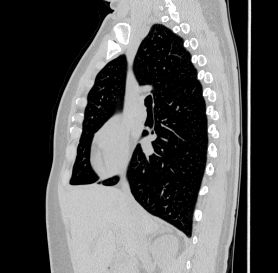
\includegraphics[width=\textwidth]{thorax/radiologist-sagital-gray.png}
        \caption{Sagital. $x=120$.}
    \end{subfigure}
    ~
    \begin{subfigure}[b]{0.3\textwidth}
        
\includegraphics[width=\textwidth]{thorax/radiologist-coronal-gray.png}
        \caption{Coroal. $y = 120$.}
    \end{subfigure}
    ~
    \begin{subfigure}[b]{0.3\textwidth}
        
\includegraphics[width=\textwidth]{thorax/radiologist-axial-gray.png}
        \caption{Axial. $z = 120$.}
    \end{subfigure}
    \caption{Visão do radiologista.}
    \label{fig:visao-radiologisa}
\end{figure}

Na Figura \ref{fig:visao-neurorradiologista}, podemos ver as fatias que estão contidas nos planos ortogonais aos eixos $x$, $y$ e $z$ e que que contém a posição $120$ de cada eixo. As fatias correspondem aos pontos de vista da direita, de cima e de trás do paciente, respectivamente.

\begin{figure}[h]
    \centering
    \begin{subfigure}[b]{0.3\textwidth}
        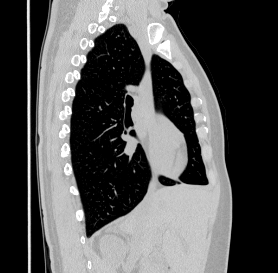
\includegraphics[width=\textwidth]{thorax/_neuroradiologist-sagital-gray.png}
        \caption{Sagital. $x=120$.}
    \end{subfigure}
    ~
    \begin{subfigure}[b]{0.3\textwidth}
        
\includegraphics[width=\textwidth]{thorax/neuroradiologist-coronal-gray.png}
        \caption{Coroal. $y=120$.}
    \end{subfigure}
    ~
    \begin{subfigure}[b]{0.3\textwidth}
        
\includegraphics[width=\textwidth]{thorax/neuroradiologist-axial-gray.png}
        \caption{Axial. $z=120$.}
    \end{subfigure}
    \caption{Visão do neurorradiologista.}
    \label{fig:visao-neurorradiologista}
\end{figure}

\section{Melhoria da visualização}
A fim de facilitar a visualização e a compreensão das fatias, podemos aplicar transformações alterar o contraste e o brilho. Nesse tipo de imagem, é comum existirem voxels com intensidade muito alta, o que pode tornar difícil visualizar a diferença entre os voxels com menor intensidade.
 
Para resolver isso, aplicamos um linear stretching utilizando uma janela e um ponto médio. A janela delimita a intensidade máxima $l_1$ e mínima $l_2$. Todo voxel com intensidade menor que a mínima recebe a intensidade mínima, todo voxel com intensidade maior que a máxima recebe a intensidade máxima e todos os outros voxels $v$ recebem intensidade \[k = \frac{2^b -1}{l_2 - l_1} (I(v) - l_1), \] sendo que $b$ é número de bits utilizado para representar as intensidades. A janela é dada por $l_2 -l_1$ e o ponto médio por $\frac{l1 + l2}{2}$.
 
Nessa tarefa, a janela é uma porcentagem da faixa de intensidades da imagem dada, e o ponto médio é uma porcentagem da intensidade máxima. Ambos, janela e ponto médio são arredondados para o inteiro mais próximo.
 
Após alterar as intensidades a fim de modificar o contraste e brilho, aplicamos um tabela de cores artificial (rainbow no caso). Para mapear cada tom de cinza para uma cor em RGB, foi utilizada a fórmula apresentada em aula. Como o tipo de imagem da IFT espera que as cores estejam em YCbCr, as mesmas foram convertidas utilizando uma função da biblioteca.
 
Na Figura \ref{fig:sull-visao-radiologista-cores} podemos ver três fatias de uma imagem de crânio dos pontos de vista do radiologista. As imagens da parte de cima mostram as fatias após a transformação nas intensidades utilizando janela de $70\%$ e ponto médio $35\%$. E nas imagens da parte de baixo podemos ver as mesmas imagens coloridas artificialmente. Os pontos de vista do neurorradiologista podem ser visto na Figura \ref{fig:skull-visao-neurorradiologista-cores}. Outros exemplos podem ser vistos nas Figuras \ref{fig:brain-visao-radiologista-cores} e \ref{fig:brain-visao-neurorradiologista-cores} para uma imagem de cérebro, sendo que na primeira temos os pontos de vista do radiologista e na segunda os pontos de vista do neurorradiologista. Para a imagem de cérebro, foi utilizada janela de $20\%$ e ponto médio de $15\%$.

\begin{figure}[h]
    \centering
    \begin{subfigure}[b]{0.3\textwidth}
        
\includegraphics[width=\textwidth]{skull/radiologist-sagital-gray.png}
        \caption{Sagital cinza.}
    \end{subfigure}
    ~
    \begin{subfigure}[b]{0.3\textwidth}
        
\includegraphics[width=\textwidth]{skull/radiologist-coronal-gray.png}
        \caption{Coroal cinza.}
    \end{subfigure}
    ~
    \begin{subfigure}[b]{0.3\textwidth}
        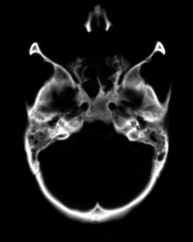
\includegraphics[width=\textwidth]{skull/radiologist-axial-gray.png}
        \caption{Axial cinza.}
    \end{subfigure}
    ~
    \begin{subfigure}[b]{0.3\textwidth}
        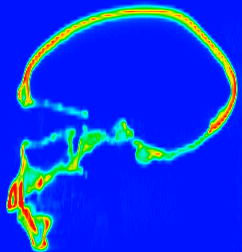
\includegraphics[width=\textwidth]{skull/radiologist-sagital.png}
        \caption{Sagital colorido.}
    \end{subfigure}
    ~
    \begin{subfigure}[b]{0.3\textwidth}
        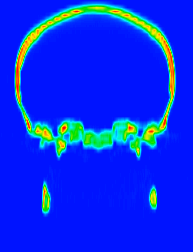
\includegraphics[width=\textwidth]{skull/radiologist-coronal.png}
        \caption{Coroal colorido.}
    \end{subfigure}
    ~
    \begin{subfigure}[b]{0.3\textwidth}
        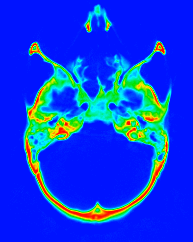
\includegraphics[width=\textwidth]{skull/radiologist-axial.png}
        \caption{Axial colorido.}
    \end{subfigure}
    \caption{Visão do radiologista da imagem de crânio com intensidades transformadas com janela de $70\%$ e nível de $35\%$. As imagens da parte de cima mostram o resultado da transformação das intensidades. As imagens da parte de baixo são o resultado da coloração artificial das imagens de cima.}
    \label{fig:sull-visao-radiologista-cores}
\end{figure}

\begin{figure}[h]
    \centering
    \begin{subfigure}[b]{0.3\textwidth}
        
\includegraphics[width=\textwidth]{skull/_neuroradiologist-sagital-gray.png}
        \caption{Sagital cinza.}
    \end{subfigure}
    ~
    \begin{subfigure}[b]{0.3\textwidth}
        
\includegraphics[width=\textwidth]{skull/neuroradiologist-coronal-gray.png}
        \caption{Coroal cinza.}
    \end{subfigure}
    ~
    \begin{subfigure}[b]{0.3\textwidth}
        
\includegraphics[width=\textwidth]{skull/neuroradiologist-axial-gray.png}
        \caption{Axial cinza.}
    \end{subfigure}
    ~
    \begin{subfigure}[b]{0.3\textwidth}
        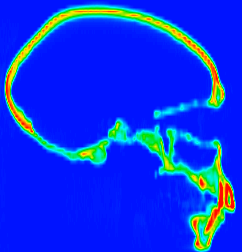
\includegraphics[width=\textwidth]{skull/neuroradiologist-sagital.png}
        \caption{Sagital colorido.}
    \end{subfigure}
    ~
    \begin{subfigure}[b]{0.3\textwidth}
        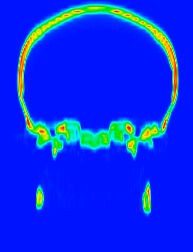
\includegraphics[width=\textwidth]{skull/neuroradiologist-coronal.png}
        \caption{Coroal colorido.}
    \end{subfigure}
    ~
    \begin{subfigure}[b]{0.3\textwidth}
        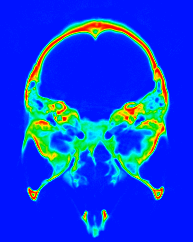
\includegraphics[width=\textwidth]{skull/neuroradiologist-axial.png}
        \caption{Axial colorido.}
    \end{subfigure}
    \caption{Visão do neurorradiologista da imagem de crânio com intensidades transformadas com janela de $70\%$ e nível de $35\%$. As imagens da parte de cima mostram o resultado da transformação das intensidades. As imagens da parte de baixo são o resultado da coloração artificial das imagens de cima.}
    \label{fig:skull-visao-neurorradiologista-cores}
\end{figure}

\begin{figure}[h]
    \centering
    \begin{subfigure}[b]{0.3\textwidth}
        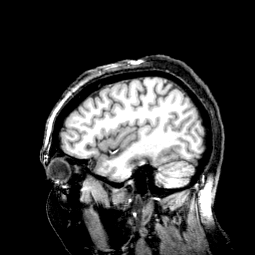
\includegraphics[width=\textwidth]{brain/radiologist-sagital-gray.png}
        \caption{Sagital cinza.}
    \end{subfigure}
    ~
    \begin{subfigure}[b]{0.3\textwidth}
        
\includegraphics[width=\textwidth]{brain/radiologist-coronal-gray.png}
        \caption{Coroal cinza.}
    \end{subfigure}
    ~
    \begin{subfigure}[b]{0.3\textwidth}
        
\includegraphics[width=\textwidth]{brain/radiologist-axial-gray.png}
        \caption{Axial cinza.}
    \end{subfigure}
    ~
    \begin{subfigure}[b]{0.3\textwidth}
        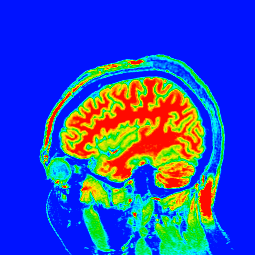
\includegraphics[width=\textwidth]{brain/radiologist-sagital.png}
        \caption{Sagital colorido.}
    \end{subfigure}
    ~
    \begin{subfigure}[b]{0.3\textwidth}
        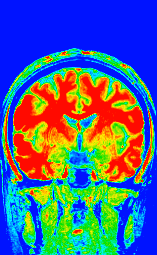
\includegraphics[width=\textwidth]{brain/radiologist-coronal.png}
        \caption{Coroal colorido.}
    \end{subfigure}
    ~
    \begin{subfigure}[b]{0.3\textwidth}
        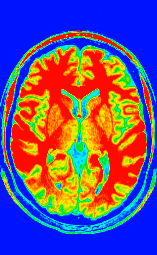
\includegraphics[width=\textwidth]{brain/radiologist-axial.png}
        \caption{Axial colorido.}
    \end{subfigure}
    \caption{Visão do radiologista da imagem de cérebro com intensidades transformadas com janela de $20\%$ e nível de $15\%$. As imagens da parte de cima mostram o resultado da transformação das intensidades. As imagens da parte de baixo são o resultado da coloração artificial das imagens de cima.}
    \label{fig:brain-visao-radiologista-cores}
\end{figure}

\begin{figure}[h]
    \centering
    \begin{subfigure}[b]{0.3\textwidth}
        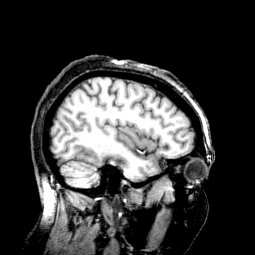
\includegraphics[width=\textwidth]{brain/_neuroradiologist-sagital-gray.png}
        \caption{Sagital cinza.}
    \end{subfigure}
    ~
    \begin{subfigure}[b]{0.3\textwidth}
        
\includegraphics[width=\textwidth]{brain/neuroradiologist-coronal-gray.png}
        \caption{Coroal cinza.}
    \end{subfigure}
    ~
    \begin{subfigure}[b]{0.3\textwidth}
        
\includegraphics[width=\textwidth]{brain/neuroradiologist-axial-gray.png}
        \caption{Axial cinza.}
    \end{subfigure}
    ~
    \begin{subfigure}[b]{0.3\textwidth}
        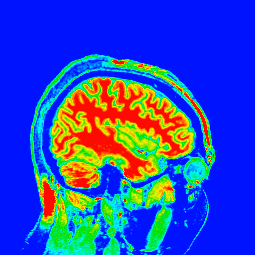
\includegraphics[width=\textwidth]{brain/neuroradiologist-sagital.png}
        \caption{Sagital colorido.}
    \end{subfigure}
    ~
    \begin{subfigure}[b]{0.3\textwidth}
        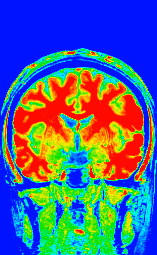
\includegraphics[width=\textwidth]{brain/neuroradiologist-coronal.png}
        \caption{Coroal colorido.}
    \end{subfigure}
    ~
    \begin{subfigure}[b]{0.3\textwidth}
        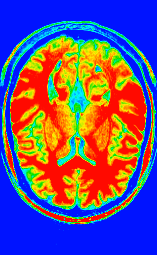
\includegraphics[width=\textwidth]{brain/neuroradiologist-axial.png}
        \caption{Axial colorido.}
    \end{subfigure}
    \caption{Visão do neurorradiologista da imagem de cérebro com intensidades transformadas com janela de $20\%$ e nível de $15\%$. As imagens da parte de cima mostram o resultado da transformação das intensidades. As imagens da parte de baixo são o resultado da coloração artificial das imagens de cima.}
    \label{fig:brain-visao-neurorradiologista-cores}
\end{figure}

\end{document}